\section{Terrestrial snake robot locomotion strategies}\label{sec:locomotion}


%--------------------------------------------------------------------------
%--------------------------------------------------------------------------

Several methods have been proposed for snake robot locomotion, most of which are inspired by nature. This part presents some of the well established strategies, as well as the newer approach, obstacle aided locomotion, which this report is based on. Finally, compliance control in snake robot locomotion is presented to open up for a comparison to what the hybrid position/force control offers.

\subsection{Traditional locomotion strategies}\label{subsec:traditional-loco}

\textbf{Lateral undulation} is the fastest and by far the most commonly implemented locomotion gait for snake robots \cite{sanfilippo2017perception}.
It is a continuous movement of the entire body of the snake relative to the ground. The locomotion is obtained by propagating sine-waves from the front to the rear of the snake \cite{transeth2006developments}, as illustrated in figure \ref{fig:lateral}.
Successful propulsion by lateral undulation requires that the snake has some grip to the surface enabling it to glide forward without slipping sideways \cite{liljeback2012review}. This again puts requirements on the friction coefficients, namely that the coefficient in lateral direction have to be greater than in the forward
direction. If the movement is conducted without slipping, every part of the body will pass through the same points on the ground.

\textbf{Concertina locomotion} is not employed on open ground, but rather in narrow spaces where the available range of motion is limited. The motion is carried out by curving the body
to create an anchor against the narrow environment (see figure \ref{fig:concertina}). The snake alternates between curving the back and front part of the body so that the front part can be stretched forward and the back part can be drawn up \cite{liljeback2012snake}.

A resembling mode of locomotion is \textbf{sidewinding}, in which one part of the body acts as an anchor while the other part is moved forward. The part that moves forward is simply lifted off the ground and displaced while the other part stays put, typically in areas with loose sand \cite{liljeback2012snake}. It can be seen as a kind of spiraling motion. Figure \ref{fig:sidewinding} gives a visual explanation of this gait.


% Rectlinear crawling?

\begin{figure}[H]
    \centering
    
    \subfloat[Lateral undulation \label{fig:lateral}]{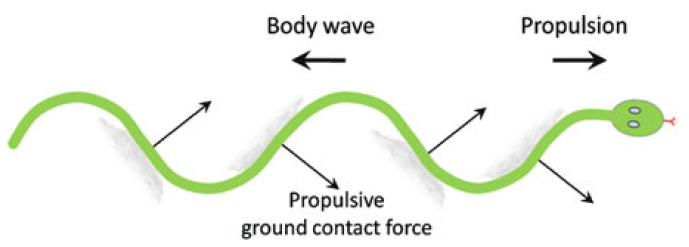
\includegraphics[clip=true, width=0.6\textwidth]{figures/theory/lateral.PNG}}

    \subfloat[Concertina locomotion \label{fig:concertina}]{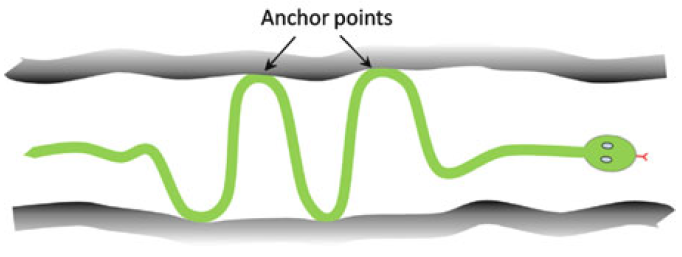
\includegraphics[clip=true, width=0.6\textwidth]{figures/theory/concertina.PNG}}

   \subfloat[Sidewinding \label{fig:sidewinding}]{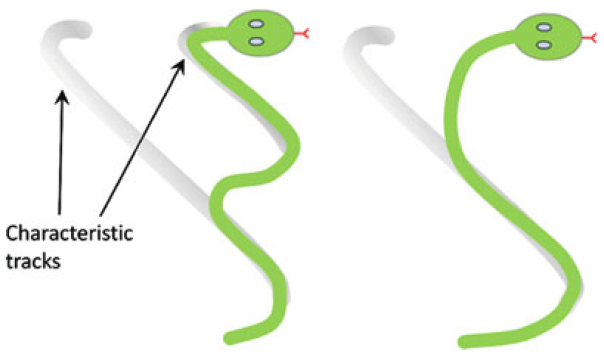
\includegraphics[clip=true, width=0.6\textwidth]{figures/theory/Sidewinding.PNG}}

    \caption{Illustration of some traditional locomotion strategies \cite{liljeback2012snake}.}
    \label{fig:traditional_locomotion}
\end{figure}


\subsection{Central pattern generators (CPGs)}

The information presented in this section is taken from \cite{ijspeert2008central}.

A central pattern generator for locomotion control is where neuroscience meets robotics. CPGs consist of neurons that produce an oscillating, rhythmic output without requiring sensory information. In nature, CPGs play an important role in periodic actions like breathing, walking and other modes of locomotion. While sensory feedback is not needed for generating the rhythms, it plays a very important role in shaping the rhythmic patterns. This is fundamental for keeping CPGs and body movements coordinated.

The method produces stable rhythmic patterns and is able to rapidly return the system to its normal rhythmic behavior after transient perturbations. Furthermore, CPG models tend to reduce the dimensionality/complexity of the control problem in that they have only a few control parameters. These parameters allow modulation of the locomotion, for instance the speed and direction or even the type of gait. This allows for higher-level controllers to circumvent the generation of multidimensional motor commands and stick to higher level control signals.

CPGs can be applied to cyclic locomotion gaits like lateral undulation, sidewinding and concertina locomotion since they are based on rhythmic patterns.

\subsection{Obstacle-aided locomotion (OAL)}\label{subsec:OAL}

Aforementioned locomotion strategies are first and foremost successful in plain, obstacle-free environments where ground friction can be used to achieve propulsion. The OAL method, on the other hand, considers flat environments with obstacles. The obstacles can be compared to the ground friction in other locomotion gaits like lateral undulation. This is because both obstacles and ground friction are used to push against. Thus, OAL can be seen as a kind of discrete special case of lateral undulation. The rest of the explanation of OAL is taken from the project work of the author \cite{AtussaProsjektoppgp}.

Instead of avoiding physical contact between the robot and obstacles, obstacle aided locomotion aims at profiting from it by using the obstacles as push-points to propel itself forward. This concept is illustrated in Figure \ref{fig:oal}. OAL was first introduced by Transeth et al. in 2008 \cite{transeth2008snake}. The motivation behind this method was based in the ability of biological snakes to utilize irregularities in the terrain for more efficient locomotion.

Liljebäck et al. \cite{liljeback2012snake} describe two major challenges related to OAL:
\begin{enumerate}
  \item It is unknown in advance when and where the snake robot will make contact with its environment.
  \item The development of a strategy for adjusting the shape of the robot so that forward propulsion is achieved in any given contact situation.
\end{enumerate}
The following hypothesis is also stated in \cite{liljeback2012snake}.
\begin{quote}
   \textit{ Obstacle-aided snake robot locomotion can be achieved by producing body shape changes where the links in contact with obstacles are rotated so that the components of the contact forces in the desired direction of motion are increased.}
\end{quote}

Holden et al. \cite{holden2014optimal} address the second challenge by formulating an optimization problem that seeks to minimize energy consumption while achieving propulsion along a user-defined desired path. The output of this optimization is the optimal motor torque inputs. In addition to a user-defined path, this method assumes that the desired link angles at the obstacles are given.

Bayraktaroglu et al. \cite{bayraktaroglu2004understanding} mention that only the trajectory of the leading link should be arbitrarily determined. Moreover, Bayraktaroglu et al. \cite{bayraktaroglu2004understanding} state that in a steady smooth motion, the trajectory of the leading link must be computed as a function of available push-points for the next contact, and the desired position and orientation of the following links are those that mimic the motion of the leading link.

\begin{figure}
    \centering
    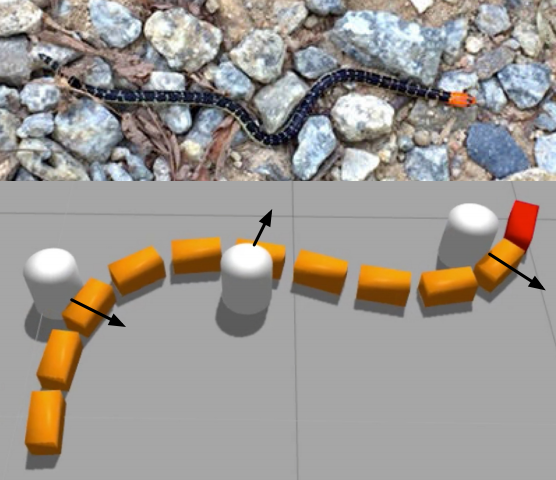
\includegraphics[width=0.6\textwidth]{figures/theory/oal.PNG}
    \caption{Obstacle-aided locomotion illustration \cite{sanfilippo2017snakesim}}
    \label{fig:oal}
\end{figure}

%--------------------------------------------------------------------------
%--------------------------------------------------------------------------


\subsection{Locomotion strategies with compliance control}\label{subsec:compliance-control}

Biological snakes cannot in any way be seen as rigid animals. Robots, on the other hand, are by default very rigid, both in the body material and actuators used.
Compliant control is fundamental when dealing with unstructured environments because it implicitly controls the energy transfer to the environment \cite{calanca2015review}.

Two main methods can be applied to snake robots to mimic the compliant and adaptive behavior between snakes and the environment they traverse. The first method is using a compliant controller for the actuators, in which they adapt a spring-like behavior. The shape-based compliance and directional compliance, among others, go under this category and are explained here. The second method is directly designing the robot with compliance, meaning that the mechanical parts are compliant.

\subsubsection{Shape-based compliance}

A very common way of controlling the shape of snake robots has been specifying the motion of each individual joint directly. This works well as long as the snake robot is traversing a flat surface without obstacles that would lead to great deviations from the planned motion.
In environments with obstacles, on the other hand, Liljebäck et al. \cite{liljeback2014compliant} proposed a specification of the motion of the robot in terms of \textit{shape control points (SCPs)}. These points specify which coordinates it is desired that the snake goes through. The points are further connected with a shape curve defined by an interpolation technique. The desired joint angles of the snake robot are eventually found by aligning a virtual robot with the shape curve and adapt its joint angles.

The work of \cite{liljeback2014compliant} is based on a model of the snake robot crawling by lateral undulation on a flat surface with circular obstacles. The compliant behavior of the snake robot is then achieved by assigning mass-spring-damper dynamics to the SCPs, making the SCPs and thus the shape curve compliant. \cite{liljeback2014compliant} propose that the adaptive behavior of the shape curve should depend on the direction of the contact force with respect to the forward direction of motion. Consequently, a natural choice is to make the shape curve highly compliant for obstructive contact forces and less compliant for propulsive contact forces.

%\subsubsection{Gait-based compliance}

%Rollinson et al. \cite{rollinson2013gait} proposed a controller in which individual joints can comply to a high-level controller built around gait parameters that specify whole-body motions. The controller is simply commanding an amplitude with a constant offset from the estimated amplitude. In the case which \cite{rollinson2013gait} call "position compliance", a positive offset causes the robot to drive forward in the gait cycle, while a negative offset causes it to drive backwards. Furthermore, the magnitude of the offset determines how hard the robot tries to push forward or backward.

\subsubsection{Directional compliance}

The disadvantage of shape-based compliance is that not all terrain features are helpful for locomotion. Some might impede the movement of the robot instead of aiding it. Because of this, a novel approach called directional compliance has been proposed by Wang et al. \cite{wang2020directional}. The approach is an improved version of the shape-based compliance controller that adapts the compliance according to the information it has about the obstacles. This information is obtained from the force measured through the joints of the robot. Thus, it is what can be called a reactive controller. Directional compliance allows the robot to selectively admit forces applied on one side and reject forces from the other side \cite{wang2020directional}.

The most substantial discovery of Wang et al. \cite{wang2020directional} is that the amplitude of the shape parameters act as an indication of the robot's forward progression. Thus, the amplitude difference from the nominal value is used to determine whether the robot should increase or decrease it's curvature at certain segments of its body. Wang et al. \cite{wang2020directional} denote admitting external forces that result in increases in curvature as positive directional compliance and admitting forces that result in decreases in curvature as negative directional compliance. The known shape-based compliance is the nominal compliance of the controller. Furthermore, a filter function is used to adapt this nominal compliance and include the two other modes.

In summary, directional compliance enables the robot to either push away from, or comply to, terrain features, based on the torque feedback measured over time \cite{wang2020directional}. This dynamical system strategy was proven successful even in a three dimensional environment. However, the main aim of this controller is utilizing obstacles the snake robot "by chance" collides with in order to avoid getting stuck between obstacles, rather than following a specific path. This means that the method is unlikely to choose the most optimal path to move forward, as is desired in OAL.


\subsubsection{Mechanical compliance}

When a robot is mechanically compliant, it typically means that it has flexible or soft mechanics. Several technologies have been explored to realise this property, like pneumatic, hydraulic, polymers etc. \cite{calanca2015review}. According to Calanca \cite{calanca2015review}, most of the implementations at the current state of the art make use of traditional electric motors with the addition of a soft element and/or a compliant controller.

Mechanical compliance allows for implicitly controlling the power transferred to the environment and to exhibit displacement if a force is applied. Furthermore, it is obvious that the response time of a mechanical compliant system always will be faster than a system with a compliant controller. The relation of compliance control to position and force control, is that an ideal position controlled system has zero compliance whilst an ideal force controlled system has infinite compliance \cite{calanca2015review}. 

\clearpage
%--------------------------------------------------------------------------
%--------------------------------------------------------------------------

